% Created 2026-10-26 lun 13:01
% Intended LaTeX compiler: pdflatex
\documentclass[a4paper]{article}

\usepackage[utf8]{inputenc}
\usepackage[T1]{fontenc}
\usepackage{graphicx}
\usepackage{longtable}
\usepackage{wrapfig}
\usepackage{rotating}
\usepackage[normalem]{ulem}
\usepackage{amsmath}
\usepackage{amssymb}
\usepackage{capt-of}
\usepackage{hyperref}
\usepackage{color}
\usepackage{listings}
\usepackage[spanish]{babel}
\usepackage[usenames,dvipsnames]{color} % Required for custom colors
\renewcommand{\ttdefault}{pcr} % MONOESPACIO CON NEGRIT
\usepackage{lastpage}
\usepackage{listings}
\usepackage{listingsutf8}
\renewcommand{\lstlistingname}{Listado}
\lstset{frame=single,inputencoding=utf8,basicstyle=\scriptsize\ttfamily,showstringspaces=false,numbers=none}
\definecolor{MyDarkGreen}{rgb}{0.0,0.4,0.0} % This is the color used for comments
\lstset{ breaklines=true, postbreak=\mbox{\textcolor{red}{$\hookrightarrow$}\space}, keywordstyle=\bfseries, keywordstyle=[1]\color{Blue}\bfseries,  keywordstyle=[2]\color{Purple}\bfseries,  keywordstyle=[3]\color{Blue}\underbar,   identifierstyle=,   commentstyle=\usefont{T1}{pcr}{m}{sl}\color{MyDarkGreen}\small,   stringstyle=\color{Purple},   showstringspaces=false,   tabsize=2,   morecomment=[l][\color{Blue}]{...} }
\lstset{literate=  {á}{{\'a}}1 {é}{{\'e}}1 {í}{{\'i}}1 {ó}{{\'o}}1 {ú}{{\'u}}1   {Á}{{\'A}}1 {É}{{\'E}}1 {Í}{{\'I}}1 {Ó}{{\'O}}1 {Ú}{{\'U}}1   {à}{{\`a}}1 {è}{{\`e}}1 {ì}{{\`i}}1 {ò}{{\`o}}1 {ù}{{\`u}}1   {À}{{\`A}}1 {È}{{\'E}}1 {Ì}{{\`I}}1 {Ò}{{\`O}}1 {Ù}{{\`U}}1   {ä}{{\"a}}1 {ë}{{\"e}}1 {ï}{{\"i}}1 {ö}{{\"o}}1 {ü}{{\"u}}1   {Ä}{{\"A}}1 {Ë}{{\"E}}1 {Ï}{{\"I}}1 {Ö}{{\"O}}1 {Ü}{{\"U}}1   {â}{{\^a}}1 {ê}{{\^e}}1 {î}{{\^i}}1 {ô}{{\^o}}1 {û}{{\^u}}1   {Â}{{\^A}}1 {Ê}{{\^E}}1 {Î}{{\^I}}1 {Ô}{{\^O}}1 {Û}{{\^U}}1   {œ}{{\oe}}1 {Œ}{{\OE}}1 {æ}{{\ae}}1 {Æ}{{\AE}}1 {ß}{{\ss}}1   {ű}{{\H{u}}}1 {Ű}{{\H{U}}}1 {ő}{{\H{o}}}1 {Ő}{{\H{O}}}1   {ç}{{\c c}}1 {Ç}{{\c C}}1 {ø}{{\o}}1 {å}{{\r a}}1 {Å}{{\r A}}1   {€}{{\euro}}1 {£}{{\pounds}}1 {«}{{\guillemotleft}}1   {»}{{\guillemotright}}1 {ñ}{{\~n}}1 {Ñ}{{\~N}}1 {¿}{{?`}}1 }
\usepackage{caption}
\usepackage{attachfile2}
\usepackage[margin=1.5cm,includeheadfoot,includehead,includefoot]{geometry}
\hypersetup{colorlinks,linkcolor=black}
\usepackage{fancyhdr}
\pagestyle{fancyplain}
\chead{}
\lhead{}
\rhead{}
\cfoot{}
\lfoot{\begin{footnotesize}alvaro.gonzalezsotillo@educa.madrid.org\end{footnotesize}}
\rfoot{\begin{footnotesize}\thepage / \pageref{LastPage}\end{footnotesize}}
\usepackage[skins]{tcolorbox}
\usepackage{multicol}
\usepackage{changepage} %ajdustwidth
\usepackage{fancybox}
\usepackage{attachfile2}
\lhead{Extraordinaria 2021 (es el \\lhead)}
\rhead{Administración y Gestión de Bases de Datos (es el \\rhead)}
\lhead{Seguridad perimetral}
\rhead{Seguridad y Alta Disponibilidad}
\usepackage{svg}
\usepackage{letltxmacro}
\LetLtxMacro{\originalincludegraphics}{\includegraphics}
\renewcommand{\includegraphics}[2][]{\IfFileExists{#2.pdf}{\originalincludegraphics[#1]{#2.pdf}}{\originalincludegraphics[#1]{#2}}}
\LetLtxMacro{\originalincludesvg}{\includesvg}
\renewcommand{\includesvg}[2][]{\IfFileExists{#2.pdf}{\originalincludegraphics[#1]{#2.pdf}}{\originalincludegraphics[#1]{#2.svg.pdf}}}
\usepackage{comment}
\excludecomment{NOTES}
\author{Álvaro González Sotillo}
\date{\today}
\title{Práctica 03: Acceso a Apache únicamente a través de VPN con Docker y wg-easy}
\hypersetup{
 pdfauthor={Álvaro González Sotillo},
 pdftitle={Práctica 03: Acceso a Apache únicamente a través de VPN con Docker y wg-easy},
 pdfkeywords={},
 pdfsubject={},
 pdfcreator={},
 pdflang={Spanish}}
\begin{document}

\maketitle
\setcounter{tocdepth}{1}
\tableofcontents

\captionsetup{font=scriptsize}

\textattachfile{/datos-luks/datos-alvaro/apuntes-clase/seguridad-alta-disponibilidad/apuntes/3/sad-03-practica-wireguard-docker.org}{} \vspace{-1em}


\setlength{\parindent}{0em}
\setlength{\parskip}{1em}

\newtcolorbox{Aviso}[1][Aviso]{
  enhanced,
  colback=gray!5!white,
  colframe=gray!75!black,fonttitle=\bfseries,
  colbacktitle=gray!85!black,
  attach boxed title to top left={yshift=-2mm,xshift=2mm},
  title=#1
}

\newtcolorbox{cuadrito}[1][Ignorado]{
  %drop shadow southeast,
  enhanced jigsaw,
  colback=white,
}


\newcommand{\StudentData}{
  \begin{cuadrito}[1\textwidth]
    \vspace{0.3cm}
    \large{
      \textbf{Apellidos:} \hrulefill \\
      \textbf{Nombre:} \hrulefill \\
      \textbf{Fecha:} \hrulefill \hspace{1cm} \textbf{Usuario:} \hrulefill \\
    }
    \vspace{-0.2cm}
  \end{cuadrito}
}

\newcommand{\StudentDataDniFirma}{
  \begin{cuadrito}[1\textwidth]
    \vspace{0.3cm}
    \large{
      \textbf{Apellidos:} \hrulefill \\
      \textbf{Nombre:} \hrulefill  \\
      \textbf{Dni:} \hrulefill \hspace{8cm} \\
      \\
      \textbf{Firma:} \hrulefill \hspace{8cm} \\
    }
    \vspace{-0.2cm}
  \end{cuadrito}
}

\newpage
\section{Objetivo de la práctica}
\label{sec:org0000000}

Tras la realización de esta práctica, el alumno será capaz de:

\begin{itemize}
\item Comprender el concepto de \emph{seguridad perimetral} y aislamiento de servicios.
\item Crear y gestionar redes puente con \emph{Docker}.
\item Desplegar un servidor \emph{Apache} aislado, sin exposición directa al host.
\item Desplegar un servidor \emph{VPN} con \href{https://github.com/wg-easy/wg-easy}{wg-easy} para dar acceso remoto seguro.
\item Verificar que un servicio solo es accesible a través del túnel \emph{WireGuard}, quedando inaccesible desde el exterior sin VPN.
\end{itemize}

Está disponible la \href{https://alvarogonzalezsotillo.github.io/apuntes-clase/seguridad-alta-disponibilidad/apuntes/3/sad-03-practica-wg-easy-apache-solo-vpn.pdf}{última versión de esta práctica en este enlace}.

\newpage
\section{Descripción del problema}
\label{sec:org0000003}

Se desea que el servidor web \emph{Apache} quede completamente aislado de la red del host. 

Únicamente los clientes que se conecten al servidor \emph{VPN} levantado con \emph{wg-easy} podrán acceder a dicho servidor \emph{Apache}.

Desde fuera del equipo, \textbf{\textbf{sin estar conectado a la VPN, NO deberá ser posible acceder al puerto 80 de Apache}}. 

El único servicio que se expondrá al host será el túnel \emph{WireGuard} (UDP 51820) y, opcionalmente, la interfaz web de gestión de \emph{wg-easy} (TCP 51821).
\section{Topología propuesta}
\label{sec:org0000006}

\begin{center}
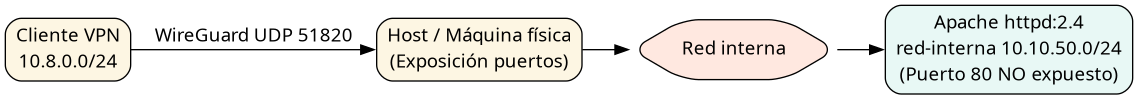
\includegraphics[width=.9\linewidth]{./media/practica-vpn-con-containers.png}
\label{}
\end{center}

\begin{itemize}
\item \texttt{red-interna}: Red puente completamente aislada. Únicamente contendrá el servicio \emph{Apache}. \textbf{\textbf{No se mapeará ningún puerto de este contenedor al host}}.
\item \texttt{wg-easy}: Contenedor conectado a \textbf{ambas} redes. Gracias a esto, podrá enrutar el tráfico procedente del túnel \emph{WireGuard} hacia la red interna donde se encuentra \emph{Apache}.
\end{itemize}

\newpage
\section{Requisitos}
\label{sec:org0000009}

\begin{itemize}
\item Equipo con \emph{Docker} instalado, para los servidores (máquina virtual)
\item Equipo con interfaz gráfica donde instalar el cliente de VPN (máquina virtual)
\item Conexión a Internet para descargar las imágenes
\begin{itemize}
\item \texttt{docker.io/weejewel/wg-easy:latest}
\item \texttt{docker.io/library/httpd:2.4}.
\end{itemize}
\item Permisos para crear redes, contenedores y modificar \texttt{sysctl}
\end{itemize}
\section{Enunciado para el alumno}
\label{sec:org000000c}

Realiza los siguientes apartados:

\begin{enumerate}
\item \textbf{Creación de red interna.} Crea la red interna \emph{Docker} donde conectar el servidor web y el servidor VPN.
\item \textbf{Despliegue de Apache.} Despliega un contenedor con \texttt{httpd:2.4} conectado únicamente a la red interna. Crea una página \texttt{index.html} personalizada y comprueba que, \textbf{sin VPN}, no es accesible desde el host.
\item \textbf{Despliegue de wg-easy.} Despliega el contenedor \texttt{wg-easy} conectado a la red expuesta al host y, posteriormente, conéctalo también a la red interna. Habilita el reenvío IP y configura los parámetros necesarios para que los clientes VPN puedan alcanzar la subred interna.
\item \textbf{Configuración del cliente VPN.} Desde el panel web de \emph{wg-easy}, crea un cliente \emph{WireGuard}, descarga su configuración o código QR e conéctalo.
\item \textbf{Comprobación del aislamiento.} Comprueba que sin estar conectado a la VPN no se accede a \emph{Apache} y, con la VPN activa, sí se accede mediante la IP del contenedor \emph{Apache} desde el cliente VPN.
\end{enumerate}

\newpage
\section{Qué se valorará}
\label{sec:org000000f}

Se entregará un documento (\texttt{PDF}, \texttt{ODT}, \texttt{DOCX} o \texttt{MD}) con la siguiente información:

\begin{itemize}
\item \textbf{Topología:} Diagrama con las redes, contenedores y flujo de tráfico (\emph{sin VPN} vs \emph{con VPN}).
\item \textbf{Despliegue:} Comandos utilizados para crear redes, lanzar contenedores y conectar \emph{wg-easy} a ambas redes.
\item \textbf{Configuración VPN:} Captura del panel web de \emph{wg-easy} con el cliente creado y/o captura del cliente \emph{WireGuard} conectado.
\item \textbf{Comprobaciones:} Mostrando la página personalizada de \emph{Apache}.
\item \textbf{Claridad y presentación:} Pasos ordenados, explicaciones razonadas y capturas legibles.
\end{itemize}
\section{Instrucciones de entrega}
\label{sec:org0000012}
\begin{itemize}
\item \textbf{Modalidad:} Individual. Solo se admitirá en pareja si así se indica expresamente en clase.
\item \textbf{Lugar de entrega:} Tarea correspondiente a esta práctica en el aula virtual del módulo.
\end{itemize}
\end{document}
